
% -----------------------------------------------------------------
% Conclusion section (insert after Results)
% -----------------------------------------------------------------
\section{Conclusion}  % -- Section VI --

% -- Paragraph 1: Summary of evaluation --
This study systematically evaluated a spectrum of methodologies for
detecting AI‐generated text, revealing both strengths and critical
limitations. Baseline algorithms achieved only moderate success and
struggled with sophisticated GPT-level outputs. In contrast, advanced
models—particularly CatBoost—substantially outperformed baselines by
capturing complex textual features, yet still encountered notable
generalisation issues on independently sourced data.

% -- Paragraph 2: Asymmetry and bias --
Results also exposed substantial asymmetry: detectors showed higher
accuracy for AI‐generated passages than for human‐written ones, implying
potential training‐data bias and underscoring the need for balanced,
representative corpora. The details can be found at \cref{fig:asymmetry}.

\begin{figure}[h!]
  \centering

  \subcaptionbox{Detect human-written accuracy against independent dataset \label{fig:image1}}{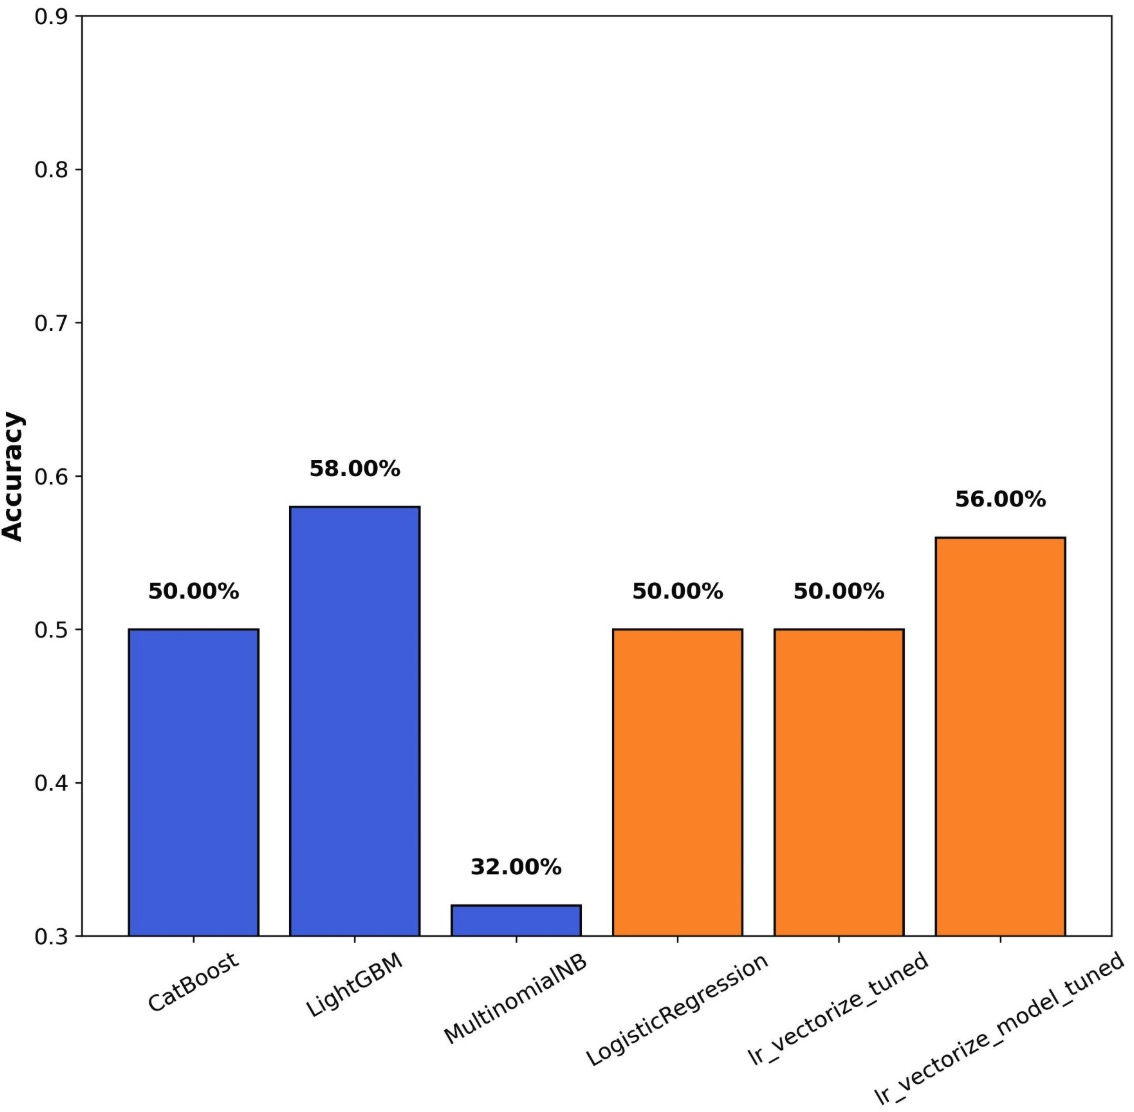
\includegraphics[width=\linewidth]{symmetric_1.jpeg}}\\
  \subcaptionbox{Detect AI-generated accuracy against independent dataset\label{fig:image2}}{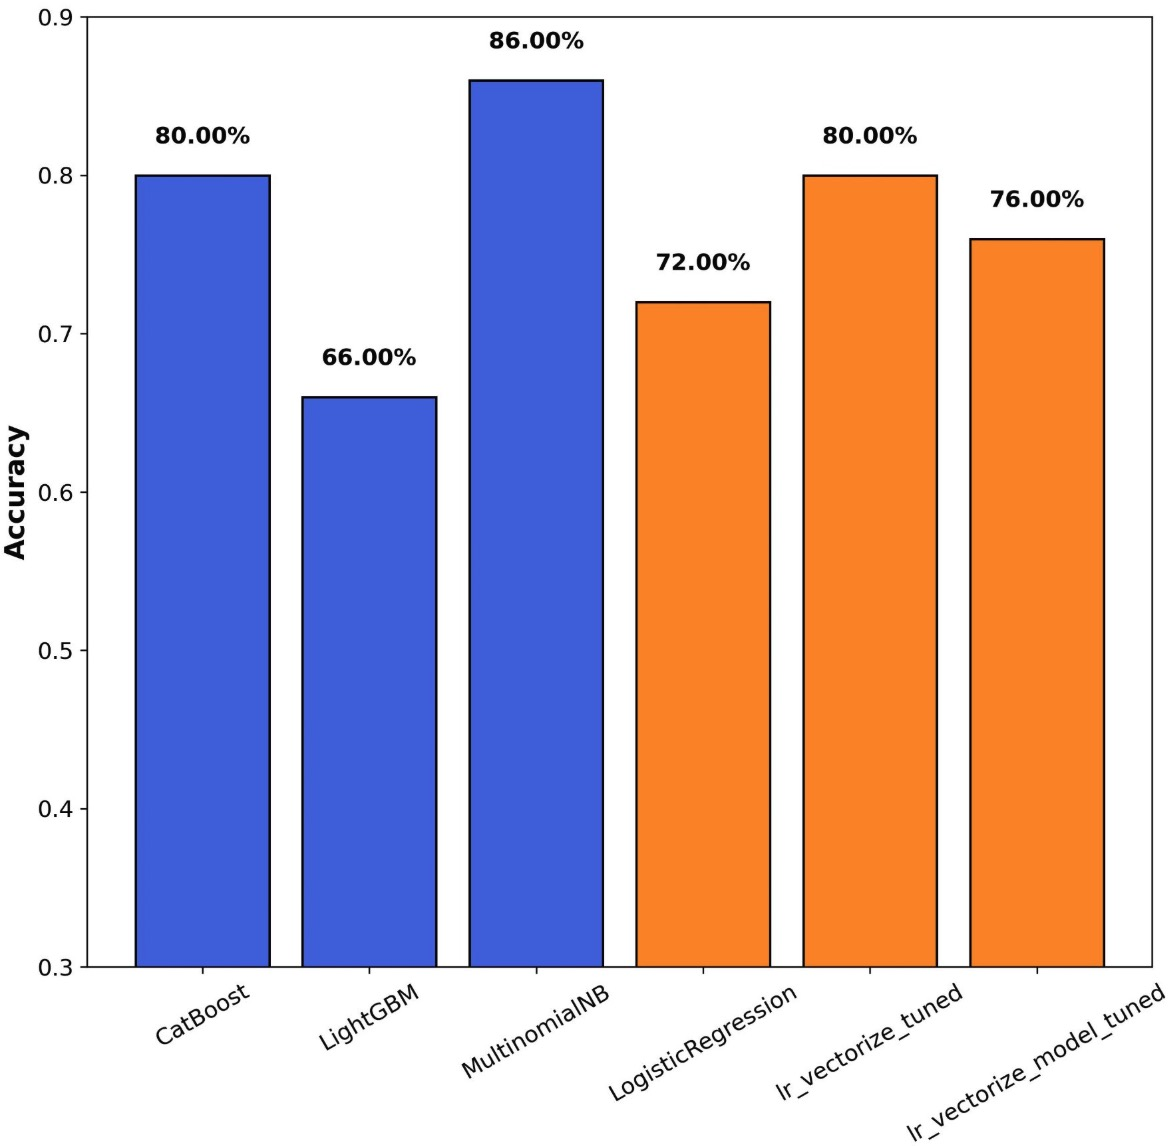
\includegraphics[width=\linewidth]{symmetric_2.jpeg}}\\
  \caption{Asymmetry accuracy}
  \label{fig:asymmetry}
\end{figure}

% -- Paragraph 3: Future directions --
Future research should prioritise robustness to emerging generative
technologies, enhanced interpretability, and ensemble strategies that
combine complementary model strengths. Expanding training datasets with
diverse, up-to-date AI‐generated samples will be essential to mitigate
domain shift and improve real-world applicability.
